\documentclass[a4paper,openright,10pt]{book}
\usepackage[spanish,es-nolists]{babel}
\usepackage[utf8]{inputenc} 
%\usepackage{lmodern}
\usepackage{amsmath}
\usepackage{amsfonts}
% \usepackage{tgbonum}
\usepackage{amsthm}
\usepackage{mathtools}
\usepackage[all]{xy}
\usepackage{float}
\usepackage[colorlinks=true,linkcolor=blue,urlcolor=blue]{hyperref} %Paquete de referencias
\usepackage{enumerate}
\usepackage{filecontents}
\usepackage{comment}
\usepackage{cite} % para contraer referencias

\setcounter{secnumdepth}{3} %para que ponga 1.1.1.1 en subsubsecciones
\setcounter{tocdepth}{3} % para que ponga subsubsecciones en el indice


\numberwithin{equation}{section}
\theoremstyle{definition}


\newtheorem{theorem}{Teorema}[section]
\newtheorem*{demo}{Demostración}
\newtheorem{corollary}{Corolario}[theorem]
\newtheorem{lemma}[theorem]{Lema}
\newtheorem{prop}[theorem]{Proposición}
\newtheorem{nota}{Nota}
\newtheorem{obs}{Observación}
\newtheorem{afir}{Afirmación}
\theoremstyle{definition}
\newtheorem{defn}{Definición}[section]
\newtheorem{conj}{Conjetura}[section]
\newtheorem{exmp}{Ejemplo}[section]

\usepackage{color}

\newcommand \numberthis { \addtocounter{equation}{1} \tag{\theequation}}
\renewcommand{\thefootnote}{\arabic{footnote}}
\bibliographystyle{ieeetr}


\begin{document}
\tableofcontents % indice de contenidos
\chapter*{Introducción}\label{cap.introduccion}

\chapter*{¿Cómo empiezo una demostración?}

\begin{itemize}
\begin{enumerate}
\item Considero que lo mas importante es saber que cosas tienes y a donde quieres llegar. 
\item Trata de hacer un bosquejo de tus cuentas.

\begin{enumerate}[a)]
\item En caso de llegar a la prueba:

\begin{itemize}
\item  Define una notación clara y que no sea redundante, a la vez no definas cosas de más. Esta es la que usaras durante la demostración.   

\item Divide la prueba en bloques. En muchas ocasiones debes demostrar pequeños resultados y juntarlos para demostrar el resultado general. Trata de definir cada bloque en tu demostración.

\item Si usas dibujos procura no referenciarlos. Usálos sólo de apoyo.  

\item Haz enfásis en los resultados utilizados, si usas algo que no ha sido demostrado, trata de probarlo para poder usarlo.
\end{itemize}

\item En caso de no llegar a la prueba con la idea que tenías trata de cambiarla. No insistas en un camino que podría no llevarte al resultado.
\end{enumerate}

\end{enumerate}
\begin{ejm}
Considerese un círculo $C$ sobre el plano, de radio 1 con centro en el origen y el trapecio isosceles $A$ de vertices sobre $C$ dados por $(1,0)$, $(-1,0)$, $(a,b)$ y $(-a,b)$. Sea $B$ un triángulo con vértices sobre $C$ de tal forma que sus lados son paralelos a los lados de $A$. Demuestra que el área de $A$ es igual al área de $B.$

\end{ejm}
Para problema anteriór se presentan dos textos, unos es una demostración y el otro no:

\begin{proof}
Empiezo dibujando la figura del problema:
\begin{figure}[!h]
	\centering
	{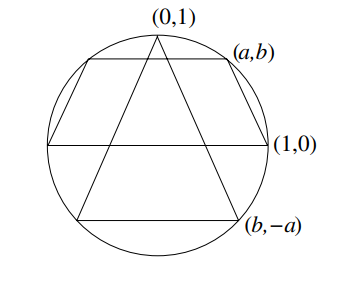
\includegraphics[width=50mm]{ejempl1.png}}
\end{figure}


Es fácil ver que que los otros vértices del tríangulo son simétricos respecto al eje x de los vertices $(a,b)$, $(-a,b)$ entonces los vertices del triángulo son  $(-a,-b)$ y $(a,-b)$ y $(0,1)$, entonces la altura del triángulo es $H=1+b$ y base $B=2a$ entonces su area es 
$$\frac{1}{2}h \cdot B =\frac{1}{2}(1+b)(2a)=(b+1)a.$$
Me doy cuenta que el trapecio tiene altura $H=b$ y base mayor igual a $B=2$, entonces su area es 
$$B \cdot H = 2b$$
entonces $2b = (b+1)a $... No resuelto.
\end{proof}
En el texto anteriór es posible notar varios errores clásicos aparte del hecho que no se concluye en nada. 

\begin{enumerate}[I)]
\item Hablar en primera persona: \textit{Yo hice}, \textit{Tomé tal cosa}, recuerda que estás escribiendo para que cualquier persona que lea el texto pueda segurilo y entenderlo, procura evitar hablar en primera persona, resta formalidad a tu demostración.

\item El uso del dibujo para la demostración: Recuerda que el dibujo \textbf{no es una prueba}, es un apoyo visual. Es claro que si dibujas mal y basas todo en el dibujo, la prueba será erronea;  Incluso si dibujas bien, el dibujo es un caso particular de entre una infinidad de posibilidades para un resultado general. 

\item Notación inconsistente: Trata de definir notación que usarás y que sea totalmente clara. En el ejemplo anteriór se define $H$ para la altúra de un triángulo y depués se usa $h$ para la misma cantidad, además $H$ y $B$ son definidas para las ay bases de triángulo y trapecio sin distinción, esto es confuso para el lector.

\item Citar resultados erroneos: Es absurdo decir que el área del trapecio está dada por el producto de su base y su altura, cláramente es incorrecto. En este ejemplo es bastante evidente pero en general puede pasar que se cite mal un resultado que no es tan obvio, es por ello que se recomienda siempre tener presente la teoría básica y entenderla.

\item La falta de conclusión: Cuando no se concluye el resultado o se llega a una prueba erronea es claro que uno de los pasos está mal o la idea general no es la correcta. Revisa detalladamente cada paso, en ocasiones un signo o una cuenta pueden sabotear todo. Si en general la idea no te lleva a ningún lado trata de cambiar de enfoque.

\item Escribir cosas como \textit{...no resulto}, \textit{...no llegué a nada} indíca que en cuanto leíste el problema empezaste a escribir improvisando y las ideas se te agotaron en un punto. No es del todo malo sin embargo te arriezgas a perder tiempo escribiendo cosas inútiles. Trata de hacer un bosquejo de la prueba antes de escribir. 

\end{enumerate}
Para la prueba comienzo separando los elementos que necesito:

\begin{enumerate}[a)]
\item Antes de comenzar la prueba debo saber que me piden y analizar que necesito para obtenerlo: Debo determinar si dos areas son iguales, la del triángulo y la del trapecio. \\

\item Determino que hipótesis y elementos tengo: Conozco los vertices del trapecio y con ellos conozco las medidas de la base mayor, base menor y su altúra, necesito determinar los vétices del triángulo para conocer su altura, su base y con ello su area. Además sé que los lados del triángulo y el trapecio son paralelos.

\item Identifico mis herramientas: Conozco la ecuación de la recta $\ell$ que pasa por dos puntos y la ecuación de las rectas paralelas a $\ell.$ También sé la ecuación de una circunferencia de radio 1.  

\item Comenzamos una idea de partida: Es posible obtener los vertices del triángulo despejando de las ecuaciones del círculo y la ecuación de la recta paralela a un lado del trapecio. 

Las cuentas anteriores las puedes realizar en una hoja aparte en caso de llegar a la solución escribe de forma ordenada la demostración.

\end{enumerate}

\begin{proof} Comenzamos observando que uno de los lados de $B$ debe de ser paralelo al segmento dado por los puntos $(-1,0)$, $(1,0)$ se sigue que dos vértices del triángulo son simétricos respecto al eje $y$ y de la misma manera dos de los lados de $B$ serán simétricos respecto al eje $y$ \footnote{No es difícil ver que si uno de los lados tiene pendiente $m$, otro tendrá pendiente $-m$ y dado que pasan por puntos simétricos se tendra que uno de dichos lados es la reflexión del otro.}, entonces la intesección de estos dos lados está dada por un punto de la forma $(0,z)$. Cómo los vértices de $B$ caen sobre $\mathcal{C}$ se concluye que $z=1$, de donde se concluye que uno de los vértices del triángulo es $(0,1).$\\

Ahora bien, consideramos el lado del trapecio cuyos vértices están dados por los puntos $(a,b)$ y $(1,0)$. Es sabido que la pendiente de la recta que pasa por los puntos $(a,b)$ y $(1,0)$ está dada por    $ \frac{b}{a-1}, $ 
entonces cualquier recta paralela a dicho lado cumplirá la ecuación 
\begin{equation}\label{eq1}
 \frac{b}{a-1}x+y_0,
\end{equation}
para algún valor $y_0 \in \mathbf{R}$. \\
Sabemos que uno de los vértices de $B$ por el que pasa la recta en la ecuación (\ref{eq1}) es $(0,1)$ llegando a que 
$$1=\frac{b}{a-1}0+y_0 \Rightarrow y_0=1.$$

Por otro lado dado que $(a,b)$ está sobre $\mathcal{C}$ se tiene que que $a^2+ b^2=1$, y con ello 
$$ b^2 = 1-a^2=(1-a)(1+a),$$ 
de donde se sigue que
\begin{equation}\label{eq2}
 \frac{b}{a-1}= -\frac{1+a}{b}.
\end{equation}
Supongamos que $(u,v)$ es el vértice del triángulo $B$ que cumple la ecuación (\ref{eq1}), usando (\ref{eq2}) se obtiene:
\begin{align*}
v&=  \frac{b}{a-1}u+1\\
&= -\frac{1+a}{b} u + 1,
\end{align*}
y finalmente tomando $u=b$ se tendrá que $v=-\frac{1+a}{b}b+1=-a$ además $v^2+u^2=(-a)^2+b^2=1$ por tanto $(u,v)=(b,-a),$ esto debido a que sólo existe una posible solución para $(b,-a).$ Por simetría concluimos que los vértices de $B$ están dados por $(0,1)$, $(b,-a)$ y $(-b,-a).$ 

Finalmente observamos que la altúra de $B$ está dada por $a+1$ y su base por $2b$ de donde su area es $$(a+1)b.$$
Por otro lado, la base mayor del trapecio tiene longitud $2$, la áltura $b$ y la base menos $2a$ entonces su area es:
$$\frac{1}{2}(2+2a)b=(a+1)b,$$
concluyendo que $A$ y $B$ tienen la misma área.
\end{proof} 




\end{itemize}
\end{document}
